% !TeX spellcheck = it_IT
\newpage

\section{Applicazioni della Computer Grafica}
\subsection{Medicina}
Nella medicina vediamo principalmente due utilizzi:
\begin{itemize}
	\item Diagnostica: sfruttare modelli 3D creati dalle immagini della MRI e CT, aumentando la leggibilità per gli umani
	\item Telemedicina e chirurgia virtuale: ad esempio la simulazione degli interventi endoscopici o preparazione di protesi dentali
\end{itemize}
\subsection{Industria}
Sfruttare il Computer Aided Design (CAD) per progettare velocemente nell'ambito industriale ed eseguire simulazioni. Ad esempio le macchine o il vestiario.

\subsection{Intrattenimento}
\subsubsection{Film}
Inizialmente effetti visivi realizzati grazie alla CGI. Si noti che bisogna distinguere tra effetti:
\begin{itemize}
	\item \emph{Visivi}: fatti in post produzione 
	\item \emph{Speciali}: fatti veri registrati dalla videocamera, ad esempio stunts o esplosioni
\end{itemize}
Poi con il tempo si è passati alla produzione di cortometraggi completamente in CGI ed infine anche lungometraggi.\\
La maggior parte sono comunque non realistici dal punto di vista degli umani, e i pochi tentativi di fare ciò sono stati fallimentari. Questo principio è rappresentato dal fenomeno dell'Uncanny Valley:
\begin{center}
	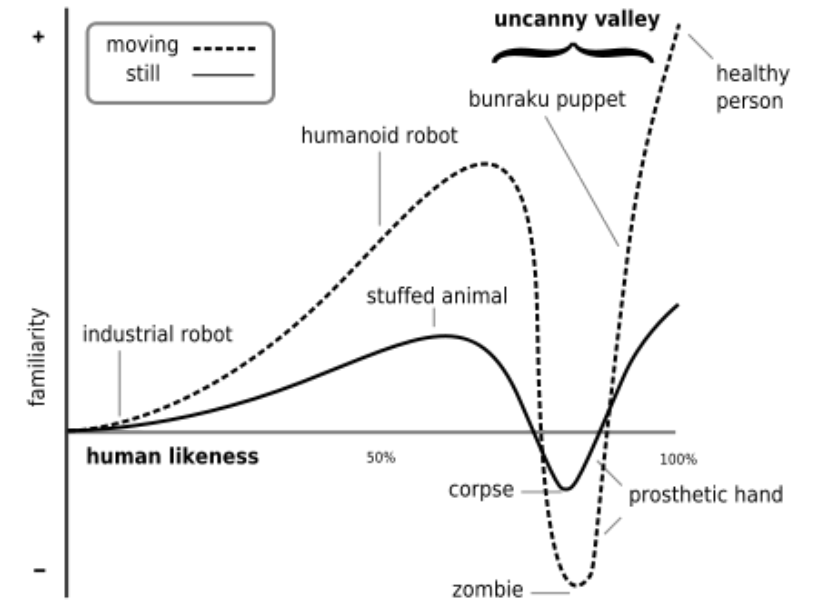
\includegraphics[scale=0.3]{uncanney_valley.png}
\end{center}
\subsubsection{Videogiochi}
Settore importantissimo per la computer grafica con un grande sviluppo.

\subsection{Beni culturali}
Un ambito relativamente nuovo per la computer grafica. Può servire per la \textbf{presentazione} (museale ad esempio), per \textbf{archiviare} pezzi artistici tridimensionali e per \textbf{studiare} (restaurazione, simulazione fisica, visualizzazione scientifica). \\
Il primo esempio di applicazione della CG è la scansione del David di Michelangelo. Una volta eseguita la scansione della statua si è creato il modello 3d dai dati grezzi e si è poi passati ad esempio al restauro.

\section{Paradigmi di renderizzazione}
Un \textbf{algoritmo di rendering} è una serie di passi che trasforma la descrizione digitale di una scena e di quattro parametri in un'\textbf{immagine raster}.\\
\begin{figure}[h]
	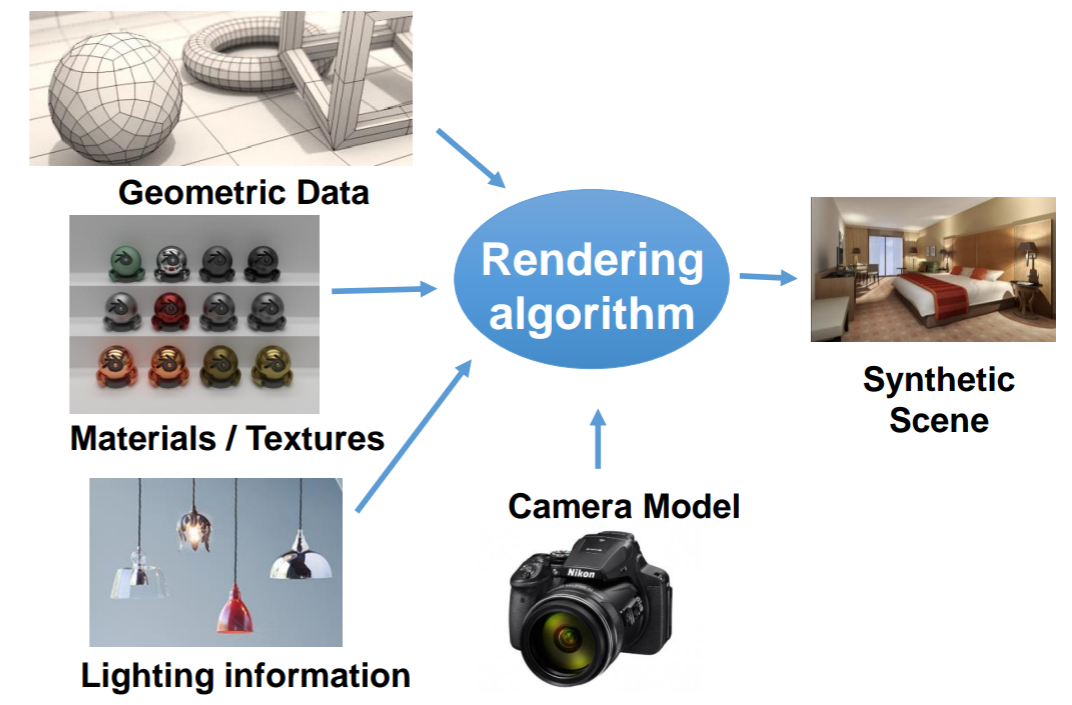
\includegraphics[scale=0.25]{rendering_algorithm.png}
	\centering
\end{figure}

\subsection{Ray Tracing}
L'idea alla base è quella di "sparare" un \textbf{raggio} dal punto di partenza e controllare se ha colpito qualche oggetto.
\begin{lstlisting}[mathescape=true]
	for each pixel p;
		make a ray r (viewpoint to p)
		for each primitive o in scene:
			find intersect(r,o)
		keep the closest intersection $o_j$
		find color of $o_j$ at p
\end{lstlisting}
Non tutti gli oggetti della scena però saranno illuminati, quindi quando un raggio interseca il punto della scena si fa partire un altro raggio che va verso la fonte di luce.\\
Se quest'ultimo incontra un oggetto vuol dire che l'oggetto è in ombra e non è raggiunto dalla luce.\\
C'è da tenere conto che la luce rimbalza un certo numero di volte, tramite il \textbf{reflection ray}. Ovviamente questo costa risorse, più si fa rimbalzare la luce e più l'immagine è realistica e costosa.\\
C'è poi la \textbf{rifrazione} di un oggetto che consiste sempre nel far partire altri raggi una volta che uno raggiunge un oggetto (ad esempio una bottiglia d'acqua).
\subsubsection{Costo}
Dipende da quanti rimbalzi ($N$) facciamo e da quante intersezioni con gli oggetti abbiamo:
\begin{equation}
	RTCost(r)=N \sum_{\forall o \in S} Int(r,o)
\end{equation}
Si noti che $Int(r,o)$ rappresenta il costo dell'intersezione del raggio $r$ con l'oggetto $o$.
\subsubsection{Primitive}
Tutto ciò che riesco facilmente ad intersecare con raggi:
\begin{itemize}
	\item Triangoli, quadrilateri, etc...
	\item Superfici implicite: sfera, geometria solida costruttiva, etc...
\end{itemize}

\subsection{Rasterizzazione}
Nella rasterizzazione (\textit{Transform \& Lighting}) proietto le primitive della scena sul mio schermo, ovvero prendo ogni \textbf{vertice} di ogni primitiva, lo proietto verso il viewpoint e vedo dove interseca la mia finestra. La linea che segna è il \textbf{proiettore}. A partire dalla proiezione dei soli vertici saprò quali pixel selezionare.\\
Il vantaggio principale è che è sufficiente proiettare pochi vertici per rasterizzare gran parte dello schermo.
\begin{lstlisting}
	for each primitive t:
		find where t falls on screen
		rasterize the 2D shape
		for each produced pixel p:
			find the color for t
			color p with it
\end{lstlisting}
\subsubsection{Primitive}
Tutto ciò che so proiettare da 3 dimensioni a 2 e rasterizzare:
\begin{itemize}
	\item Punto
	\item Segmento
	\item Triangolo
\end{itemize}
\subsubsection{Pipeline}
\begin{enumerate}
	\item Identifico le proiezioni delle primitive sullo schermo
	\item Trovo l'area da rasterizzare
	\item La computo
\end{enumerate}
\begin{figure}[h]
	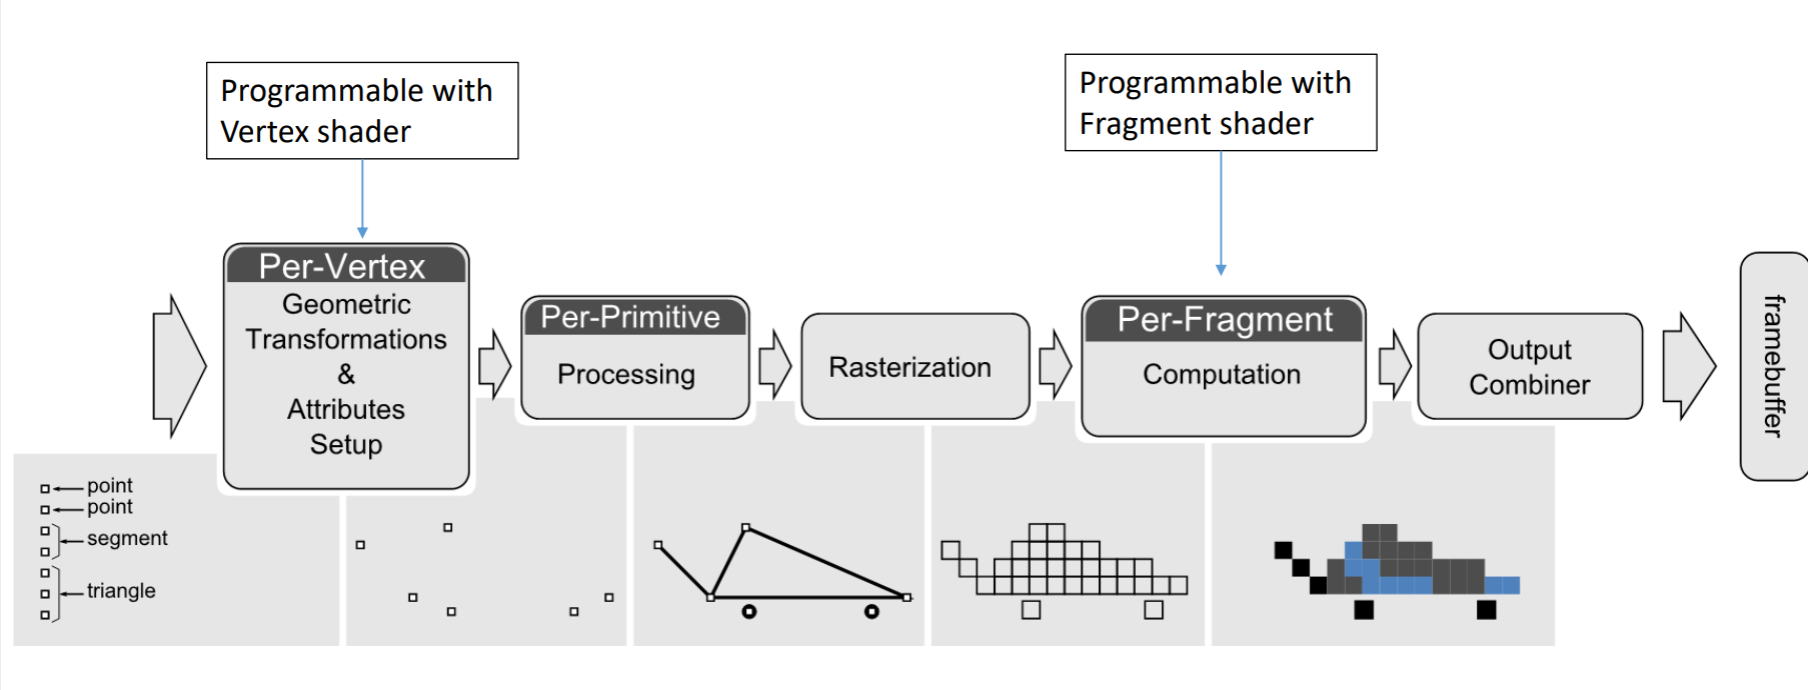
\includegraphics[scale=0.25]{rasterization_pipeline.png}
	\centering
\end{figure}
\subsubsection{Punto}
\subsubsection{Linea}
Conoscendo i due vertici trovare tutti i pixel che la coinvolgono. Utilizzando l'equazione della rette si applica il seguente codice:
\begin{lstlisting}
	RasterizeH(x0,y0,x1,y1){
		m = (y1-y0)/(x1-x0)
		x=x0;
		y=y0;
		do{
			pixel(x,y)=0
		}
	}
\end{lstlisting}
\subsubsection{Triangoli}
Dati i tre vertici, se i lati passano per il centro del pixel allora questo viene illuminato. Questo ci garantisce che non ci sia ambiguità in caso di triangoli adiacenti, poiché non "litigheranno" per lo stesso pixel.
\subsubsection{Costi}
È composto dal costo della trasformazione dei vertici e il costo di rasterizzare la primitiva p in proporzione alla sua dimensione sullo schermo:
\begin{equation}
	%TODO
\end{equation}
\subsection{Confronto}
Ancora ad oggi il metodo della \textit{rasterizzazione} è il più popolare.\\
I vantaggi del \textit{ray-tracing} sono i seguenti:
\begin{itemize}
	\item Algoritmo più semplice concettualmente
	\item Ottimo per effetti grafici complessi di \textbf{alta qualità}
\end{itemize}
mentre quelli della \textit{rasterizzazione}:
\begin{itemize}
	\item Complessità più controllabile in quanto non serve tutta la scena in ogni momento della renderizzazione: ogni primitiva lavora per conto suo ed è quindi più facilmente parallelizzabile
	\item Funziona meglio con i dati dinamici (oggetti che si muovono sulla scena)
	\item Più \textbf{controllabile} e \textbf{veloce}
\end{itemize}
Uno dei motivi principali per cui ancora oggi la rasterizzazione è più popolare è per come affronta il problema dell'\textbf{Hidden Surface Removal}.
\subsubsection{Combinazione}
La soluzione vincente è quella di usare entrambi gli approcci: la \textbf{rasterizzazione} per disegnare gli oggetti della scena e il \textbf{ray-tracing} per elaborare luci ed ombre.